\subsection{Decision Tree} \label{sec:tree}
Von der Problemstellung und der anschließenden Datenanalyse ausgehend, ist der Algorithmus des Entscheidungsbaumes (engl. \glqq Decision Tree\grqq) sehr gut geeignet. Der Grund diesbezüglich liegt im Vorgang der Diagnostik. Hierbei werden die Fragen schrittweise abgearbeitet. Die Resultate der Fragen werden dabei in zwei möglichen Formen \glqq Trifft zu\grqq{} und \glqq Trifft nicht zu\grqq{} bewertet. Diese Art des Vorgehens ähnelt dabei der Funktionsweise des Entscheidungsbaum-Algorithmus. In dieser Arbeit wird hierzu nun der von \textit{sklearn} implementierte Algorithmus verwendet. Um die Trennschärfe noch weiter zu Verbessern wird eine der Parameter der maximalen Tiefe $d$ des Entscheidungsbaumes $T$ definiert. Die maximale Tiefe $d(T)$ wird dabei für $n$ Merkmale auf $d(T) = n-1$ gesetzt. Dies ermöglicht es, dass für jedes Merkmal maximal eine Entscheidung getroffen wird und führt zur gewünschten Verbesserung der Trennschärfe.

Bereits aus der Datenanalyse (siehe Kapitel \ref{sec:analysis}) ist ersichtlich, dass die Zuordnung der Klassen anhand des Merkmals \textit{result} eindeutig durchführbar ist. Dies bestätigt der in Abbildung \ref{fig:tree_graph} dargestellte Aufbau des Entscheidungsbaumes. Dieser wurde dabei mit Hilfe von 20 Trainingsdaten durch das Framework \textit{sklearn} automatisch generiert. Dabei wählt der Algorithmus ebenso das Merkmal \textit{result} als Entscheidungsmerkmal zur Klassifizierung.

\begin{figure}[h!]
\centering
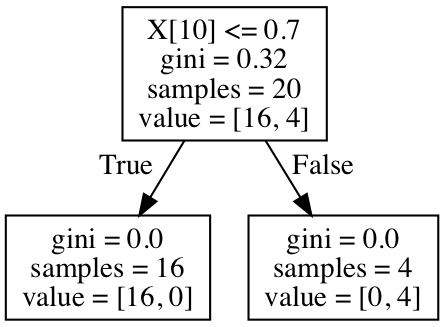
\includegraphics[scale=0.7]{graphs/tree_graph.png}
\caption{\em Automatisierter Aufbau des Decision Tree durch \glqq sklearn\grqq{} durch Prüfung der Merkmale}
\label{fig:tree_graph}
\end{figure}